\begin{titlepage}
%	\includepdf[pages=-]{front_cover.pdf}

% The easiest way to cope with RuG font requirements is just use your favorite text editor (word, libre) and export that to PDF. Remember to set your page to B5! There's a .doc file attached.
	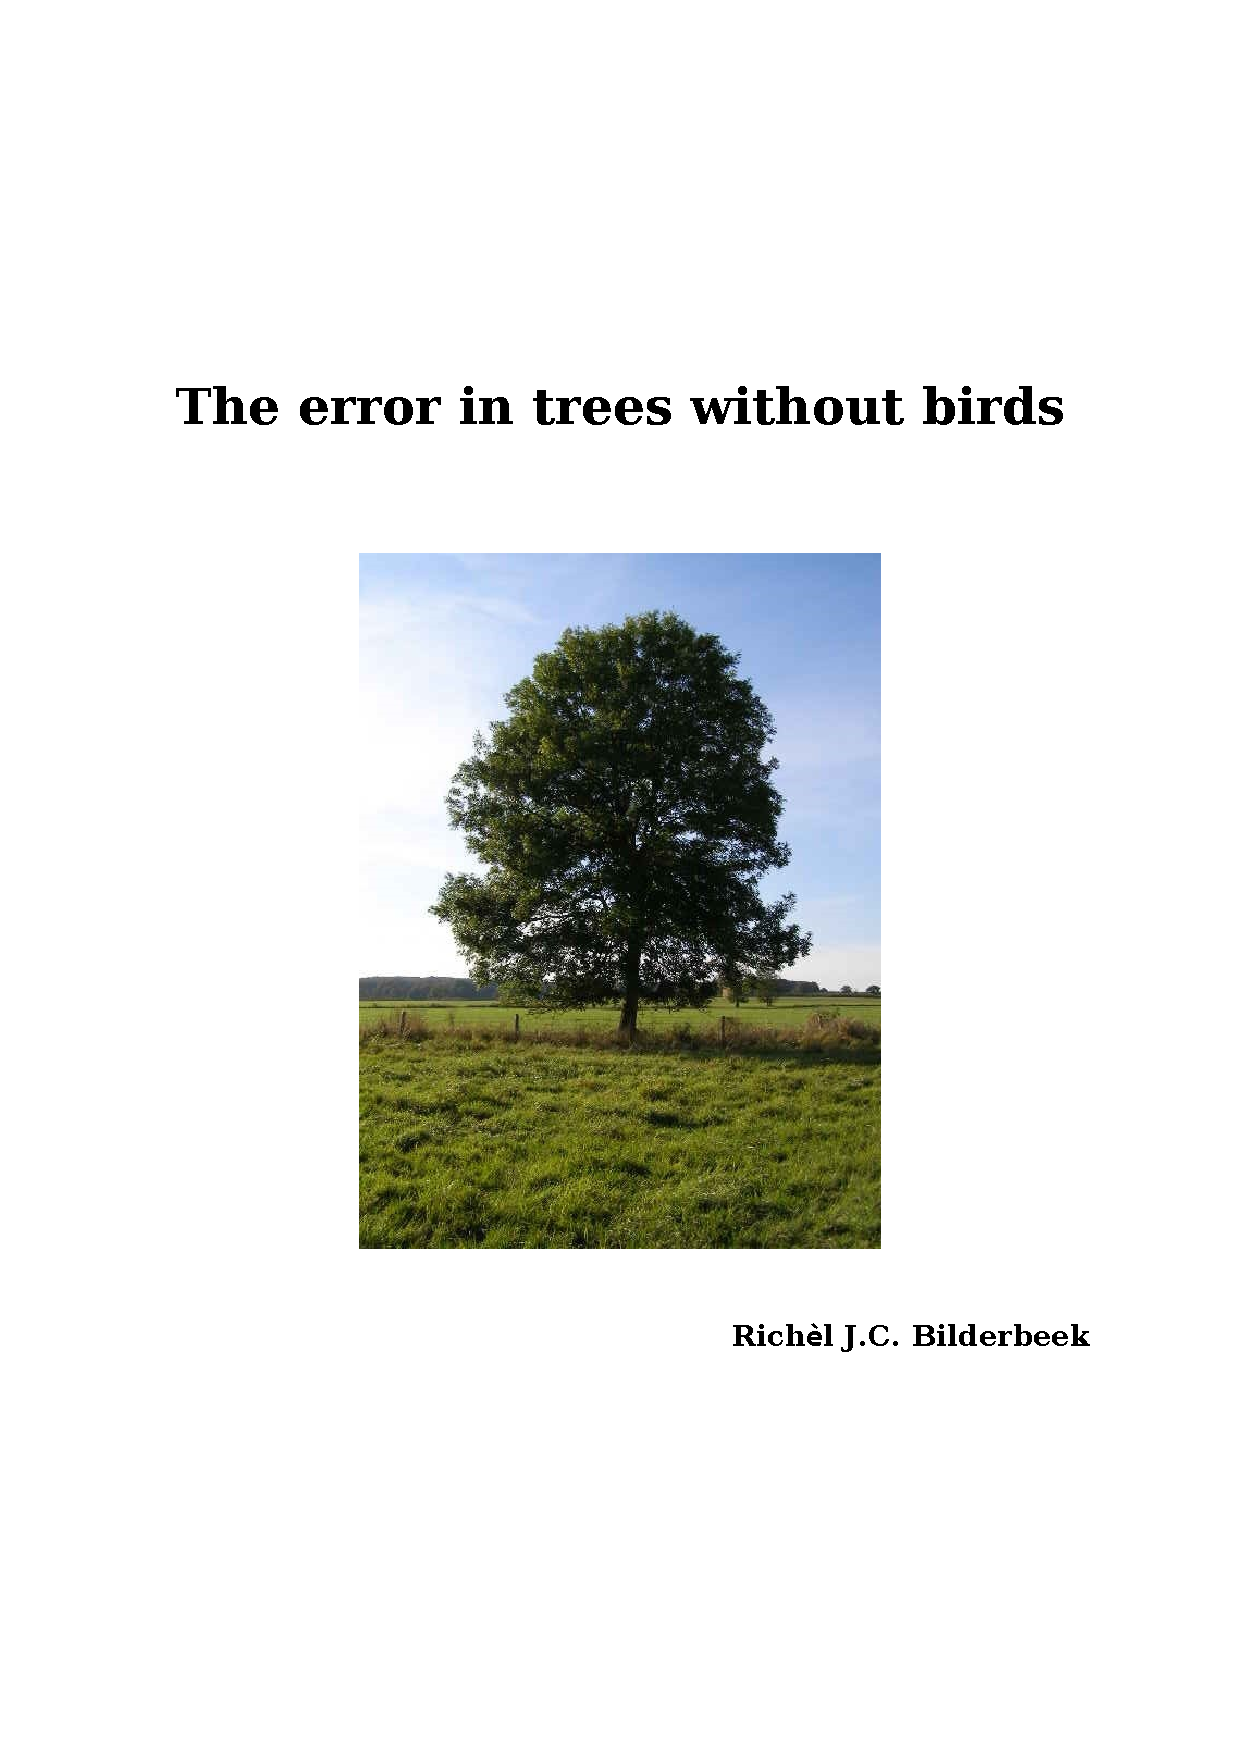
\includepdf[pages=-]{title/firstpage.pdf}
	
	
	%%%%%%%%%%%%%%%%%%%%%%%%%%%%% Book information page %%%%%%%%%%%%%%%%%%%%%%%%%%%%%%%%%%%%%
	
	\newpage \thispagestyle{empty}
	\vspace*{3.9cm}%{4.7cm} was 5.7, save 2 for FSC logo
	
	
	\begin{figure}[!h]
		
\includegraphics[width=\textwidth]{images/frontmatter/rugr_fse_logoen_rood_cmyk.pdf}
	\end{figure}
	
	\vfill
	\begin{figure}[!h]
		
\includegraphics[width=0.5\textwidth]{images/frontmatter/gelifes_header_600x320.png}
		
\includegraphics[width=0.4\textwidth]{images/frontmatter/tece_logo_2.png}
	\end{figure}
	\noindent
	{\small 
		Zernike Institute PhD thesis series 2020-09 \\
		ISSN: 1234-5678\\
		ISBN:	123-45-678-9012-3 \\
		ISBN: 123-45-678-9012-3 (electronic version) \\
		\\
		The work described in this thesis was performed in the research group 
    Theoretical \& Evolutionary Community Ecology at the University of Groningen, the Netherlands. \\
		\\
		Cover design: Rich\`el J.C. Bilderbeek\\
		Cover image: Common ash (\textit{Fraxinus excelsior}), photo by Brian Green. 
    This is the first tree shown at \url{https://en.wikipedia.org/wiki/Tree}.
		\\
		An electronic version of this dissertation is available at: \\
	  \verb;https://github.com/richelbilderbeek/thesis;. \\
		Print: Ridderprint | www.ridderprint.nl \\
		} 	
	
	
	\clearpage
	
	
\includepdf[pages=-]{title/titlepage.pdf}
	
\end{titlepage}
